%\chapter{Simulations: Time and Trajectory using the optimizer algorithm}
%\chapter{Laser Simulations for the Race 1 at the World Cup Series 2018 Hyéres, France}
\chapter{%Simulations: for time and trajectory for the Race 1 at the World Cup Series 2018 in Hyéres, France}
Results of the time and trajectory for the Race 1 at the World Cup Series 2018 Hyéres, France} \label{sec:simulations}

Sailing regattas for Olympics classes take place all around the world and one event that features them is the World Cup Series. This competition is a series of regattas organized at various cities around the world during a year and it is the Word Sailing Organization  responsible to regulate this event. This means that the races follow most of the policies that govern the Olympic Sailing Events.
One series of the World Cup Series 2018 was hosted by Hyéres, France during April. \par \noindent
\textit{SAP Sailing Analytics}\textsuperscript{\textregistered} recorded all the details of each race, including participants, times, GPS trajectories and wind measurements and it is open access \cite{SAPsailingana}. Because of this, one race during this event is a reference for the estimated results using the algorithm developed on this research and for the \acrshort{wrf} wind model developed.  \par 

The aim of this chapter is to compare the optimization results, time and trajectory, for a laser race from 3 sizes granularity configurations of the wind model.
The first configuration of the wind model assumes a step time of 1 hour, this means that all the wind properties remain constant for 1 hour. The second assumes a step time of 10 minutes (\textit{1/6 hr}) and for the last, the algorithm uses the wind measures from \cite{SAPsailingana}. In each configuration, the legs under the upwind mode compare the results from the optimization when the heading-direction is the port and when it is at starboard. \par 

This chapter is organized into three sections, the first section describes the location and area of the race with the parameters mentioned during the previous chapter. The next section shows the inclusion of the \acrshort{wrf} wind model area with the course area and last part presents the results of the tests described before. The order of these results follows the same order introduced in this chapter.   \par 

%\section{Set-up Parameters for the algorithm}\label{sec:details about the place} Set-up parameters and location details about of the race

\section{Integration of the Race: Location and Configuration for the initialization parameters of the algorithm}\label{sec:details about the place}

The laser race to simulate took place in the World Cup Series 2018 in Hyères, France during April. The identification label of the race is \textit{R1}, and it is a trapezoid course with 5 legs, 2 of them sailed at upwind-downwind mode and the last under direct wind mode. The event features all the Olympic classes organized in 5 areas around the bay as shown in figure \ref{fig:course_area}, the area within R1 took place in \textit{Echo} and its diameter is approximately \textit{1.5 NM} equivalent to 2963 meters, with its center at 43º 04.144'N,006º 11.913'E. %43,4.144;6,11.913
 \par 
 
The wind area defined uses the parameters from section \ref{sec:SailinArea_WindModel} and the courses areas to limit the wind model area before knowing the locations of the buoys. Figure \ref{fig:Courses_LatLon} shows the locations of the areas for the competition in \textit{Lat-Lon coordinates in degrees} while figure \ref{fig:Courses_XY} is the same figure but with \textit{XY coordinates in meters}. In both figures, the red lines are the limits of each course and the green squares denote the limits of the \acrshort{wrf} wind model used during this simulation. The green square at the center shows the center coordinates from all the courses areas. First, the algorithm uses the area inside these limits, and once the buoys coordinates are available, then it defines the area of each leg which limits the location of the stage-points at each leg. \par
%is this area included in the definitions of the space constraints for each stage inside the leg. \par
%figure shows both areas and the limits of the \acrshort{wrf} wind model used during this simulation. 


%\begin{figure} [hbt!]
%    \centering
%    \includegraphics[width=0.4 \linewidth]{images/CourseAreaFR.png}
 %   \caption{Course Areas of the World Cup Series 2018 in Hyéres, France \cite{france_laser}}
%    \label{fig:course_area}
%\end{figure}%
\begin{figure} [hbt!]
  \centering
  \subfloat[Courses Areas Locations using Lat-Lon (deg)Coordinates.] {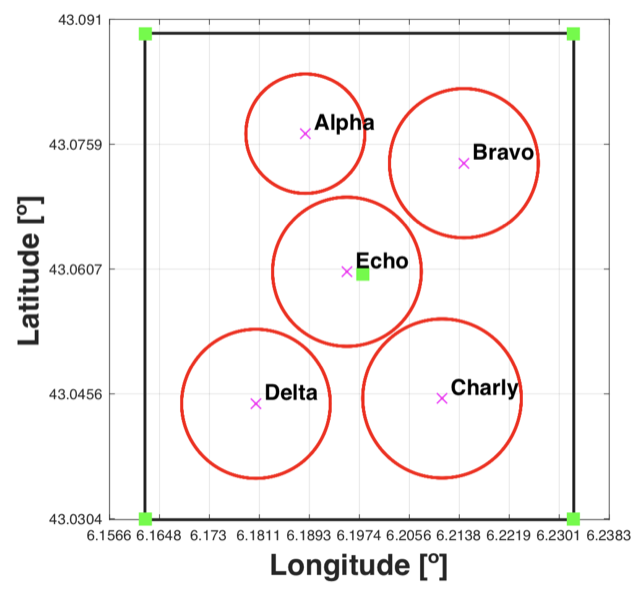
\includegraphics[width=0.47 \linewidth]{images/FR_LatLon.png} \label{fig:Courses_LatLon}}
  \hfill
  \subfloat[Courses Areas Locations using X-Y Coordinates (m).] {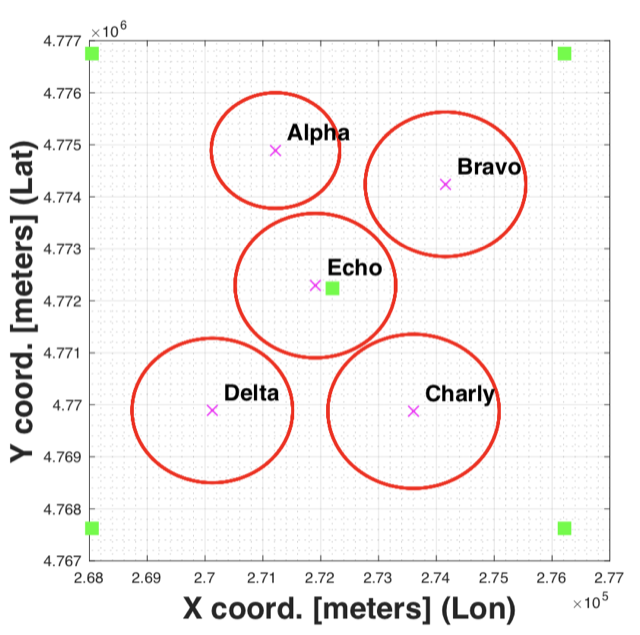
\includegraphics[width=0.45\linewidth]{images/FR_XY.png} \label{fig:Courses_XY}}
  \caption{Courses Areas of the World Cup Series 2018 Hyéres, France} %$\Delta t$ =5s and
\label{fig:course_area}
\end{figure}

The courses of the competition adjusted the wind model area in the \textit{XY coordinates}, for the height (\textit{Z coordinate}) this optimization algorithm only considers the first two levels. Their corresponding heights, in meters, are \textit{7.5} and \textit{25}. %Using the velocities of the first level it compares the wind measurements from the race. 
The comparison between the \acrshort{wrf} wind model and the wind's measurements of the race uses only the first level because both heights are approximately at the same. However, the velocities for the optimal path are at the \acrshort{ce}, at a shorter height, and they are getting using equation \ref{eq:wind_h}. \par  

%The \acrshort{ce} of the laser is calculated at  is the distance from the deck to the sail foot (boom above deck)
First, the calculation of the \acrshort{ce} for the laser's sail uses the \textit{40\%} of the height's sail and then adds the height of the sail foot, from the top of the deck \cite{pennanen2015optimal},\cite{philpott1993yacht},\cite{claughton1998sailing}. % from the top of the deck, 
As a result, the \acrshort{ce} is at \textit{2.68 meters} from the sea level.
Figure \ref{fig:wrf_diffH} shows how the height influences the velocities, both figures are over the same area and time. The figure uses \textit{Lat-Lon coordinates}, and it includes all the courses shown in figure \ref{fig:Courses_LatLon}, the black arrows show the divergence of the wind field and the direction from where it comes. \par  \noindent

The velocities at \textit{7.5 meters}, \ref{fig:wrf7_5} have a larger magnitude at the center of the area with a larger divergence than those at \textit{2.68 meters} where the magnitude in average is smaller, except for the left-bottom corner of figure \ref{fig:wrf_268} where even the divergence is much larger than in the rest of the area. The reason for such behavior is that of the power relation (exponent \acrshort{kappa} of equation \ref{eq:wind_h}. This equation describes the ratio between heights at power \acrshort{kappa}, to the ratio between their velocities, therefore, the wind behavior at that area does not appear at 7.5 meters. %This wind behaviour does not appear at \textit{7.5 meters} at it is related to the \ref{eq:wind_h} which uses a power relation (exponent \acrshort{kappa}) to describe the ratio change in heights to the ratio change on velocities. 

\begin{figure} [hbt!]
  \centering
  \subfloat[WRF wind map at 7.5m height] {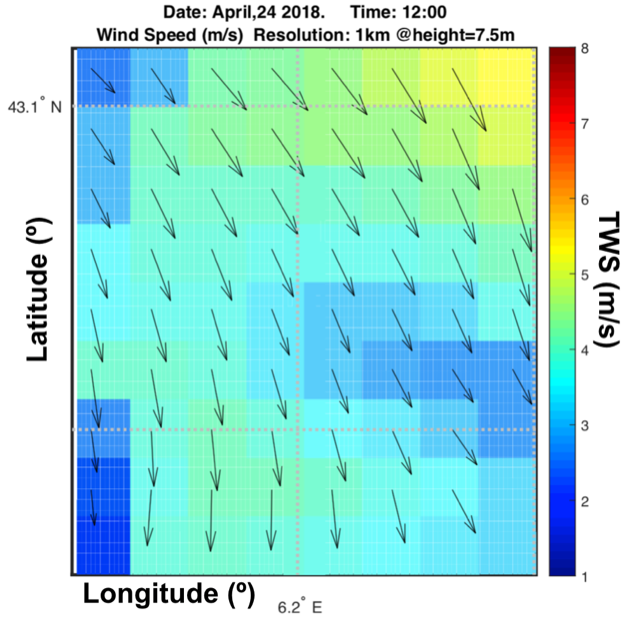
\includegraphics[width=0.43 \linewidth]{images/7_5M12_Wo_course_windarea.png}%7_5M12pm_course_wind_area.png}
  \label{fig:wrf7_5}} 
  \hfill
  \subfloat[WRF wind map at 2.68m height] {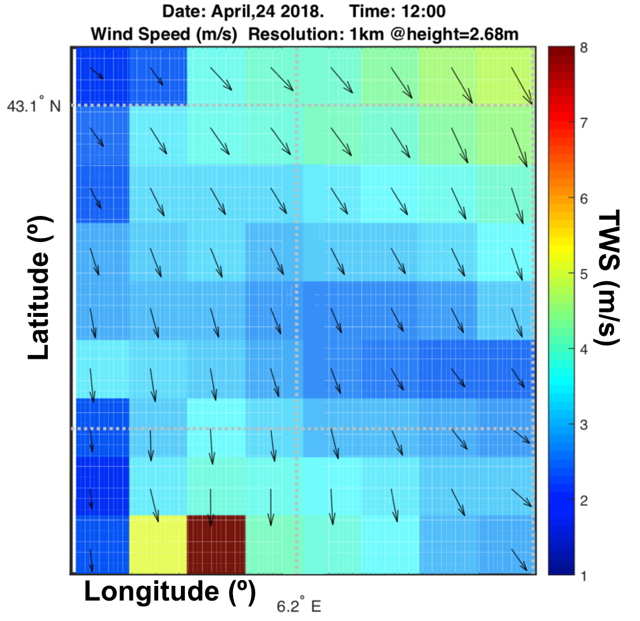
\includegraphics[width=0.43\linewidth]{images/2_68M12pm_course_windarea.png} \label{fig:wrf_268}}
  \caption{Wind map at 2 different heights over the Courses Areas of the World Cup Series 2018 Hyéres, France} %$\Delta t$ =5s and
\label{fig:wrf_diffH}
\end{figure}

Another dimension to consider is the time because the same area could be subject to distinctive wind patterns as time went by. For this, the algorithm requires an estimated time at which the race could start and use equation \ref{eq:time_window} to set the \textit{time window}. The \textit{time window} describes the distribution of the \acrshort{v_tw} and its \acrshort{b_tw} and presented with a variation of the polar plot where the axes refer to the angle and velocity ranges. Assuming that the competition started at \textit{12:00 hrs}, it defines the \textit{time window} as follows. 

\begin{equation} \label{eq:timeW_comp}
    \textrm{Time window} = \big[10:00,16:00 \big]
\end{equation}

At 7.5 meters height the range of velocities and angles estimated for the race, which has a duration approximately of one hour, is less than 6 m/s (11.66 kn) while its angle range is between [90,180] degrees with  dominated directions from [120,180] degrees. Figure \ref{fig:75compass13} shows both ranges, the circles represent the velocities, the bigger the circle, the larger the velocity. The distribution of the \acrshort{v_tw} over the map on the courses areas, figure \ref{fig:75mwindarea12} and \ref{fig:75mwindarea13}, show it has a range value between 3 m/s to 5 m/s, and at the end of the race, the model \acrshort{wrf} predicts to have higher velocities one hour after the race starts. Thus, the maps show the distribution of the wind at that specific time while figure \ref{fig:75compass13} involves all the values and changes from \textit{12:00}hrs to \textit{13:00}hrs.% Most of the measurements related to wind are taken at least at 7.5 meters or higher.
The 7.5 height is a reference because for wind measurements this is the minimum height recommended and the most used. 
\begin{figure} [hbt!]
  \centering
  \subfloat[WRF Wind map at 12:00 hrs.] {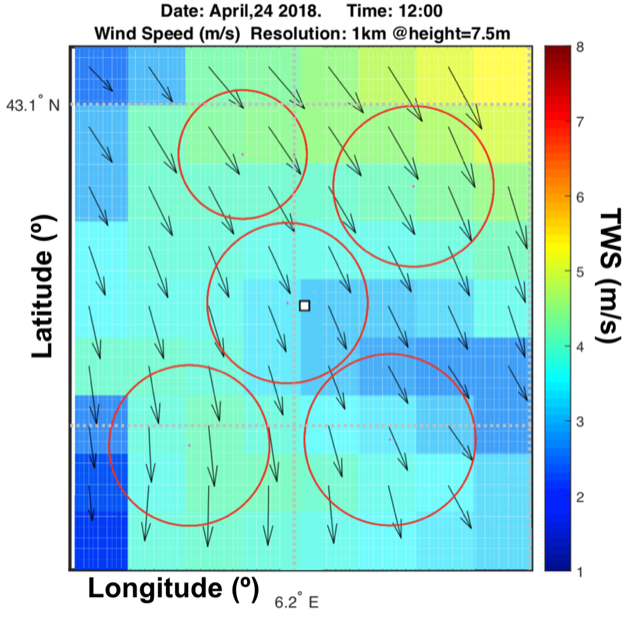
\includegraphics[width=0.31 \linewidth]{images/7_5M12pm_course_wind_area.png} \label{fig:75mwindarea12}}
  \hfill
  \subfloat[WRF Wind map at 13:00 hrs.] {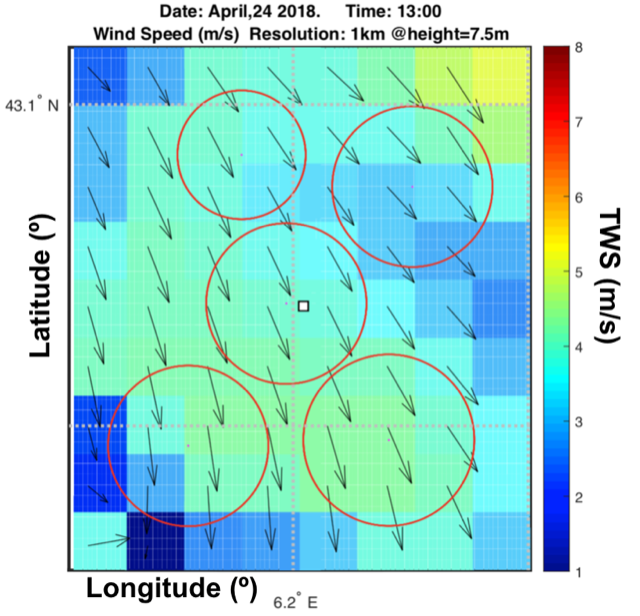
\includegraphics[width=0.33\linewidth]{images/7_5M13pm_Wcourse_wind_area.png} \label{fig:75mwindarea13}}
    \hfill
  \subfloat[Wind Directions from 12:00 to 13:00 hrs.] {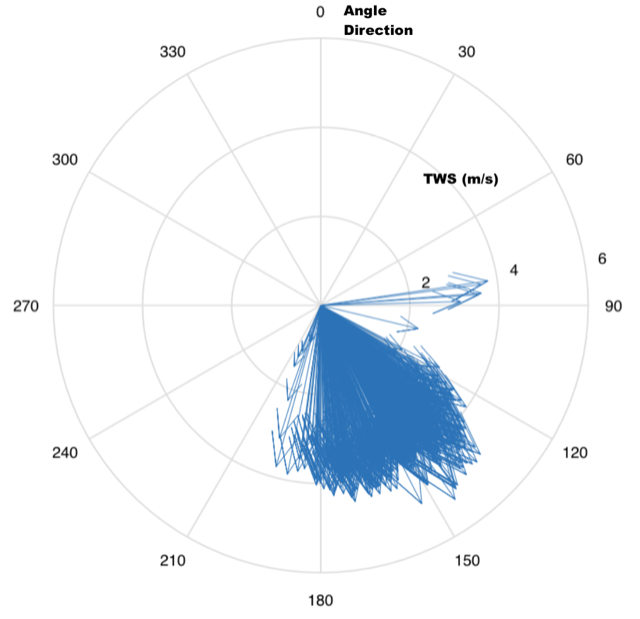
\includegraphics[width=0.31\linewidth]{images/7_5winDri12_13.png} \label{fig:75compass13}}
  \caption{WRF Wind Area at 7.5m with the courses from the World Cup Series 2018 Hyéres, France} %$\Delta t$ =5s and
\label{fig:75mwindarea12_13}
\end{figure}

At the \acrshort{ce} height, the wind velocities pattern and angle range show similar outcomes than at 7.5 meters contrarily the velocities at this height are smaller. The speeds estimated at the end of the race are higher than initially similarly, figure \ref{fig:268_mapCA_13h} shows that the divergence of the wind field is also higher at the end. The beginning of the race, figure \ref{fig:268_map_12hrs}, shows 2 areas with higher velocities and the central area of the competition has a wind speed around 3m/s. \par 
\begin{figure} [hbt!]
  \centering
  \subfloat[WRF Wind map at 12:00 hrs at CE height.] {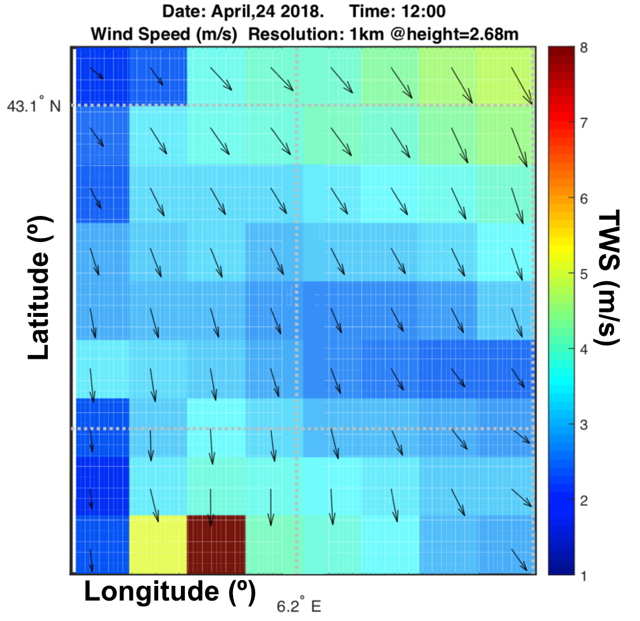
\includegraphics[width=0.33 \linewidth]{images/2_68M12pm_course_windarea.png} \label{fig:268_map_12hrs}}
  \hfill
  \subfloat[WRF Wind map at 13:00 hrs CE height.] {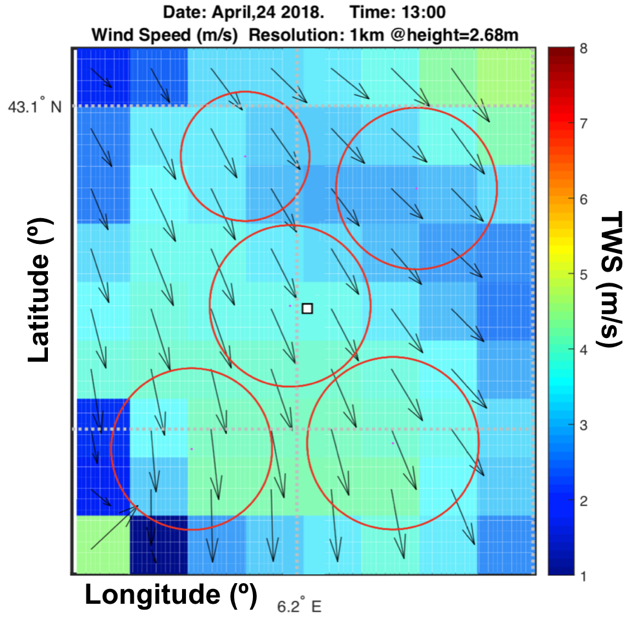
\includegraphics[width=0.33\linewidth]{images/2_68M13pm_Wcourse_windarea.png} \label{fig:268_mapCA_13h}}
    \hfill
  \subfloat[Wind Directions from 12:00 to 13:00 hrs at CE height.] {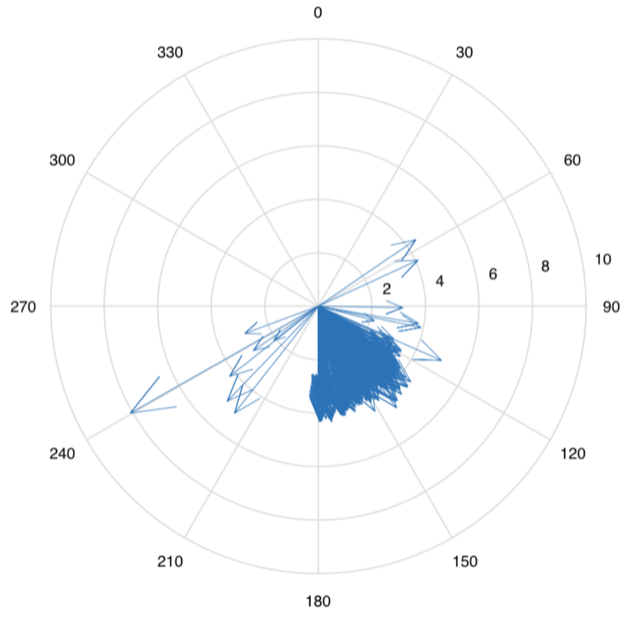
\includegraphics[width=0.31\linewidth]{images/268winWRF_Dir_12_13.png} \label{fig:268compass_12_13}}
  \caption{WRF Wind Area at CE height within the courses from the World Cup Series 2018 Hyéres, France} %$\Delta t$ =5s and
\label{fig:268_WSWD12_13hr}
\end{figure}
In fact, the range of speed velocities expected (\acrshort{v_tw}) during the race, from 12:00 to 13:00 hr, is close to 4m/s similar to the ones at 7.5 meters. However, figure \ref{fig:268compass_12_13} shows that at this height some areas experience larger velocities compared with the velocities at 7.5 meters and with various directions, the angle range is from [80,240] degrees. The concentration of the speed and angles is equivalent to the 7.5-meter height. 

After completing the adaptation of the wind area to the course areas from the World Cup Series 2018 in Hyères, France,  and define the time window, the simulations only requires the locations of the buoys. The buoy's locations are in \textit{XY coordinates}, instead of \textit{Lat-Lon coordinates} hence the velocity and displacement use the same base units. \par %the displacement and velocity use the same base units. 
The race to simulate is the \textit{R1}, and it has a trapezoid shape with 5 legs. The leg 1 and 3 are in the upwind mode, both finished at buoy 1 but started at other location. The \acrshort{wrf} wind area used is larger than the area covered by the buoys as shown in figure \ref{fig:weather_xy_bouys}, the red squares are the buoys locations with its identification label in blue. The magenta line represents the limit of the \textit{Echo} course, previously explained, and the 2 black dots are the locations of the grid points where the wind model estimates the wind's velocity ($V_{tw_{i,j}}$). \par \noindent
\begin{figure} [hbt!]
    \centering
    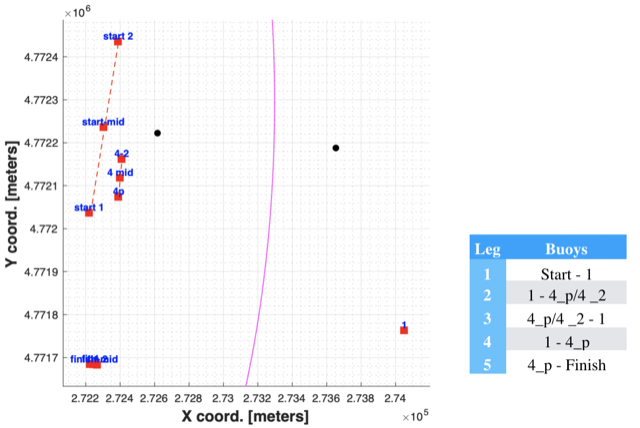
\includegraphics [width=0.75 \linewidth] {images/buoys_leg.png} %{images/ibouys_xy_Clim_xyTWS.png}
    \caption{Buoys location in \textit{XY coordinates} for R1 for the Laser Class at the World Cup Series 2018 in Hyéres, France}
    \label{fig:weather_xy_bouys}
\end{figure}

The figure shows 2 lines a start line and a second line that uses the buoys labeling with the number 4, and a third smaller line for the finish buoys at the bottom of the figure. This algorithm uses also the midpoint of all the lines to estimate the optimal path. The start line is the longest of them, 430 meters while the end line is the shortest with 42 meters, and the other line is about 90 meters. Because of the configuration of the racecourse, and these lines the length of the first leg varies from 1793 to 1850 meters with and its angle goes from 98.5\degree to 112 \degree respect to the North. To find the optimal path, the algorithm discretizes the lines using 3 points the north, the middle and the south point. The length of each leg and the angle direction for each point configuration are in figure \ref{fig:buoysLines_DistAng}. \par  

\begin{figure}[hbt!]
    \centering
      \subfloat[Using the north points of the race lines.]{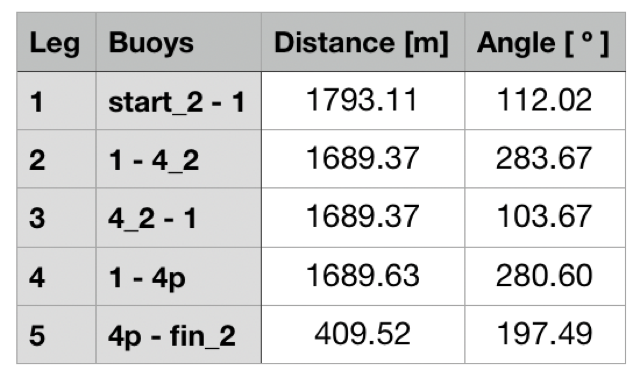
\includegraphics[width=0.27 \linewidth]{images/North_points_leg.png} \label{fig:north_point}}
  \hfill
        \subfloat[Using the middle points of the race lines. ]{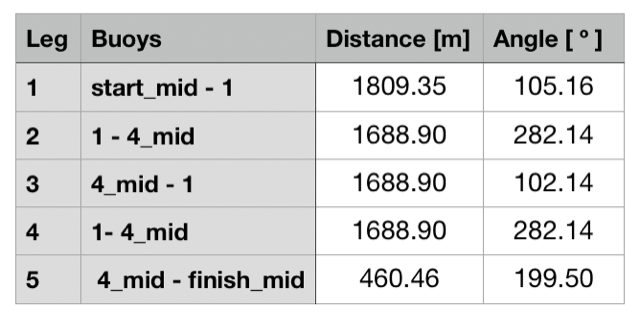
\includegraphics[width=0.33 \linewidth]{images/Middle_points_leg.png} \label{fig:middle_point}}
  \hfill
        \subfloat[ Using the south points of the race lines.]{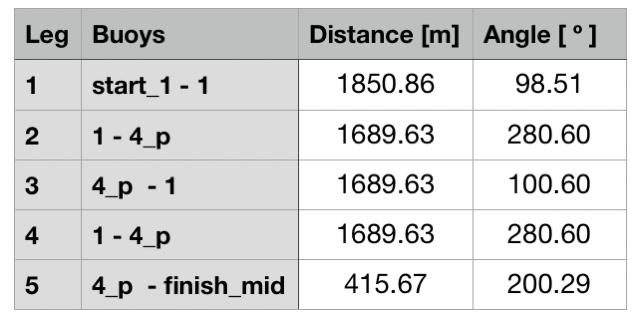
\includegraphics[width=0.32 \linewidth]{images/South_points_leg.png} \label{fig:south_point}}
\caption{Length's leg and angles using the respective points of the each race line.}
\label{fig:buoysLines_DistAng}    
\end{figure}

The race course is smaller compared with the area defined for the wind and to estimate the average wind properties to which the race is subject to the limits have to include more grid points. A visual representation of the wind characteristics and the racecourse in \textit{XY coordinates} on meters is in figure \ref{fig:weather_bouys_detaila}. To have enough information about the wind over the racecourse, the number of grid points is at least 12. Using these grid points showed by arrows on figure \ref{fig:zoom_xy_wind_bouys} the wind properties estimated, \acrshort{v_tw} and \acrshort{b_tw}, are 4m/s with a wind range angle about [120,180] degrees, figure \ref{fig:compass_ibouys}. The figure also shows that a straight-line path for leg 2 is at least subject to 3 diverse wind conditions. Because of these, for the optimal path prediction the algorithm uses more points at the \textit{Y-axis}, thus one additional level at each side. \par 

\begin{figure} [hbt!]
  \centering
  \subfloat[Buoys location for R1 and courses within the WRF model]{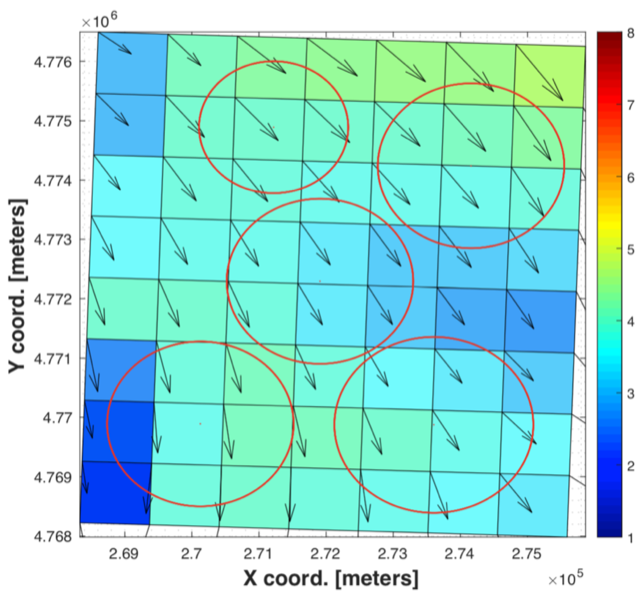
\includegraphics[width=0.32 \linewidth]{images/xy_wind_courses_bouys_12pm_75m.png} \label{fig:xy_wind_ibouys}}
  \hfill
  \subfloat[Close up to the Buoys location for R1.] {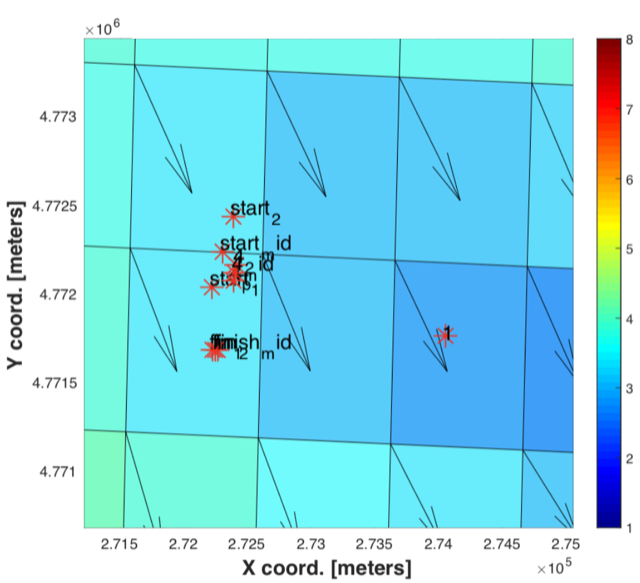
\includegraphics[width=0.32\linewidth]{images/zoomXY_ibys_12pm_75m.png} \label{fig:zoom_xy_wind_bouys}}
    \hfill
  \subfloat[Wind Directions from close up to the buoys location for R1.] {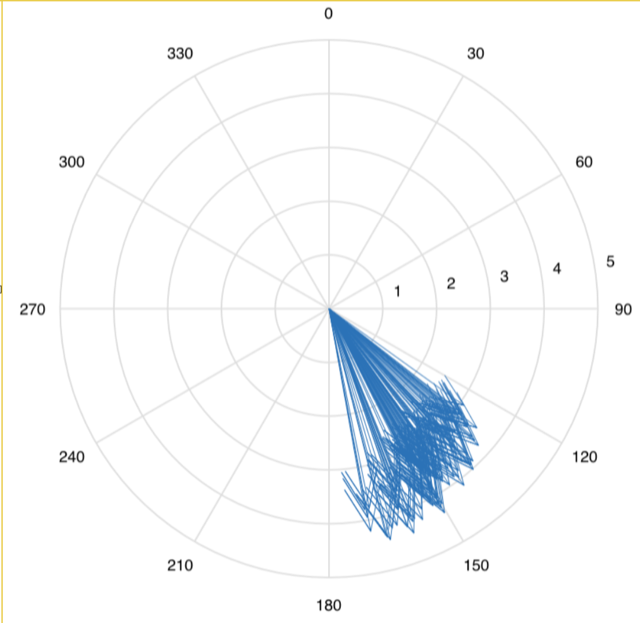
\includegraphics[width=0.3\linewidth]{images/compass_12_13_75m_ibys.png} \label{fig:compass_ibouys}}
  \caption{Buoys location in meter using \textit{XY coordinates} and the WRF wind model for World Cup Series 2018 Hyéres, France} %$\Delta t$ =5s and
\label{fig:weather_bouys_detaila}
\end{figure}
%However, the \acrshort{ce} of the sail is at a lower height and to obtain the velocities there equation \ref{eq:wind_h}  %the \acrshort{WRF} wind model.
After defining the racecourse with its legs and its location respect to the wind area, the following section shows the results for the simulations performed. The sailing races for Olympic classes are subject to changes, however, with the information previously provided is possible to limit the area and define the time window. The locations of the buoys tunes this setup and parameters, for example, the wind conditions can change the locations of the racecourse at areas not considered initially by the courses areas, hence, the locations of some buoys are out of the initial course area.
%are  using only the initially locations of the courses the   %the location of the courses at the beginning shows its location and limits, and because of the wind conditions, the racecourse is not within it. \par \noindent 
Changes on the start time and location of the racecourses happen frequently during the development of these events. Despite these changes, which could occur one day before the competition, they don't have a negative impact on the definitions of the model. Since the last changes or information provided contributes to locate precisely the race and then define the space limits on each leg.\par
%using these values and its corresponding speeds in equation , the value of \acrshort{kappa} at each coordinate is obtained. 
\section{The Scenarios to Simulate the Minimal Time Path} \label{sec:wind_area_and_course_area}
This section shows the results of five scenarios where the time step and space dimension have distinct configurations. The first and simplest scenario assumes a uniform and constant wind field, the rest of the scenarios varies the time step and grid configuration. %it uses the same grid space configurations while the last one uses the wind measurements from the race taken at 5 locations.
The minimal time path for the race results from the minimal time path for each leg. Therefore, the algorithm analyzes the 3 buoys/legs configurations shown in figure \ref{fig:buoysLines_DistAng}. On each leg, it also tests the tack direction at the start, to port or to starboard at various angles. These means that the algorithm on each leg uses at least 12 initial conditions for its optimization, at least 2 start angles by side (sub-paths). The reason for them is not only to review the convergence of the solution but also to eliminate the local optimal solutions. \par 
%The initial conditions of the first scenario uses the average values of the \acrshort{v_tw} and \acrshort{b_tw}, and they are uniform over the race area. The next three scenarios have the same initial conditions of the wind but using different time steps, This model varies over the space and uses a grid size. The las scenario uses the wind measurements from the race, with.\par \noindent
The first scenario is a constant and uniform wind field. The second has a time step of 60 minutes or 3600 seconds, this means that the wind conditions remain constant during this time but varies over the space. The third scenario is like to the previous scenario but it has a time step of 30 minutes or 1800 seconds. The next scenario uses the full resolution of the \acrshort{wrf} model, %The similar to h a the second case uses the time resolution of the model, then the 
the time step is about 10 minutes or 600 seconds. All these 3 scenarios vary over the space and have a grid size of 1km in \textit{XY coordinates}. The last scenario uses the wind measurements from the race taken at 5 locations with a sampling rate of 20 Hz. The race started at 12:11 hrs on April 24, 2018; this time defines the initial conditions of the wind while the algorithm with the buoys coordinates determines the space constraints for each leg. %the space constraints of the each leg locations of the sailboat is determined by the algorithm and the buoys coordinates.  \par % the third scenario  

\subsection{Constant and  Uniform Wind %Time Step of 1 Hour
}

The properties of this scenario are the simplest used in this research. The value of the  \acrshort{v_tw} was 5.61 m/s or 10 kn with and \acrshort{b_tw} equal to 108 \degree respect to the North. Figure \ref{fig:cnstWind_mtp_upw} shows the two legs on upwind mode, Leg 1 and Leg 3, on these legs the start position uses the line discretization represented by 3 points. Another parameter is the tacking direction at the start, to port or to starboard, these means there are at least 12 initial values of the variables to optimize. The figure shows the best solution by point and by direction, this means that there are 6 paths presented. The thickest lines are the paths with the minimal time of the best two solutions for each leg. \par 

\begin{figure} [hbt!]
  \centering
  \subfloat[Buoys location for R1 and courses within the WRF model]{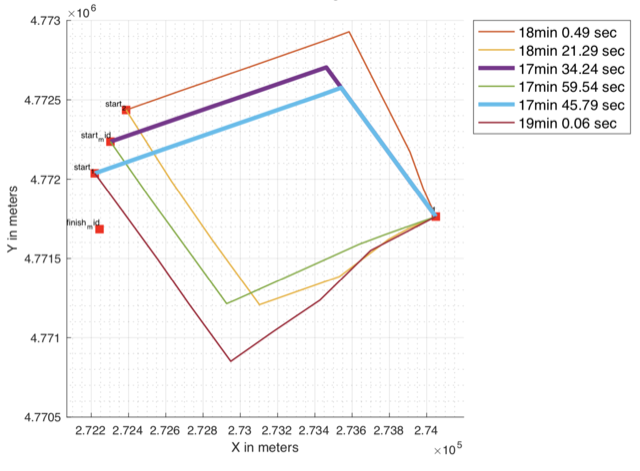
\includegraphics[width=0.44 \linewidth]{images/WindConst_Leg1_mC.png} \label{fig:l1_cnstWind}}
  \hfill
  \subfloat[Close up to the Buoys location for R1.] {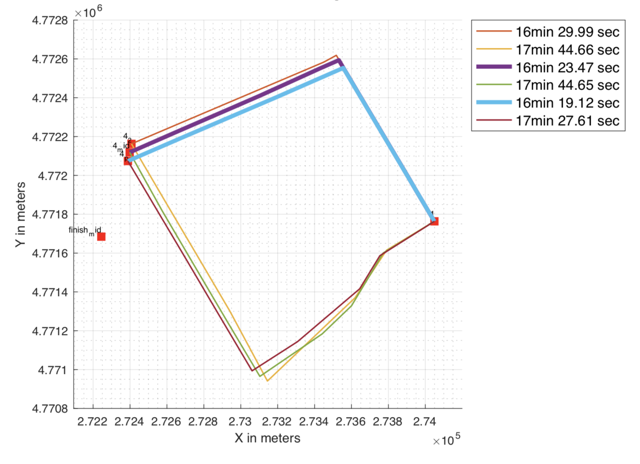
\includegraphics[width=0.44\linewidth]{WindConst_Leg3_mC.png} \label{fig:l2_cnstWind}}
  \caption{Buoys location in meter using \textit{XY coordinates} and the WRF wind model for World Cup Series 2018 Hyéres, France} %$\Delta t$ =5s and
\label{fig:cnstWind_mtp_upw}
\end{figure}

For this scenario and on the upwind mode, the minimal time path follows one tack direction after the start and it goes to the North but the star point is at the middle point of the start line and alternative start is at the south point. For the rest of the legs, the straight line gives the minimal time path, figure \ref{fig:mtp_constWind} shows the minimal time path for the race and the conditions used in this scenario. For this scenario the minimal time path is 53 minutes with 10.38 seconds, the first leg starts at the midpoint while the third leg is at the south point, the angle of tacking to arrive at the next buoy is the same for both legs. \par  

\begin{figure} [hbt!]
  \centering
  \subfloat[Total Time and Time per Leg ]{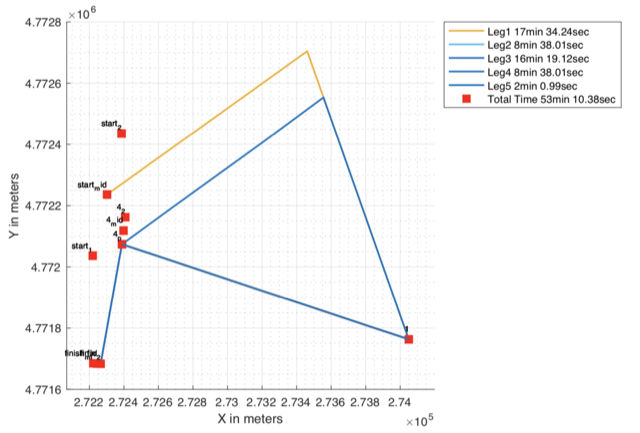
\includegraphics[width=0.53 \linewidth]{images/WindConst_mtp1_mC.png}} \label{fig:windConst_times}
  \hfill
  \subfloat[Wind Conditions] {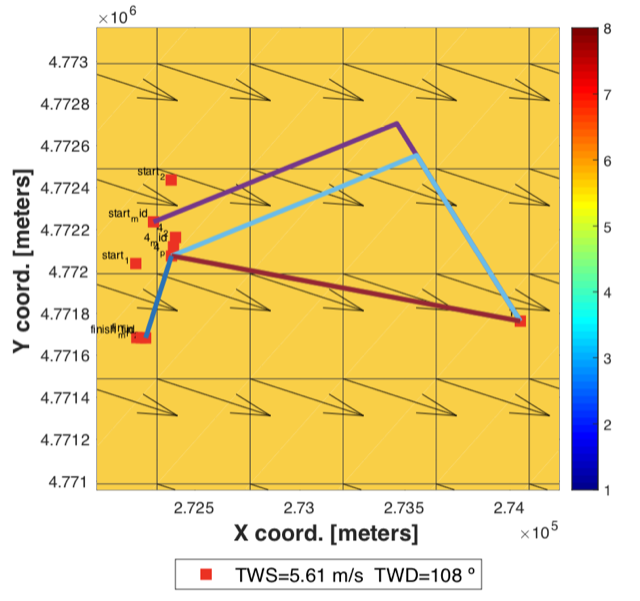
\includegraphics[width=0.38 \linewidth]{constwind.png} \label{fig:windConst_prop}}
  \caption{Minimal Path for a Constant Wind of 5.61 m/s at 108 \degree} %$\Delta t$ =5s and
\label{fig:mtp_constWind}
\end{figure}

%\begin{figure}[hbt!]
    %\centering
    %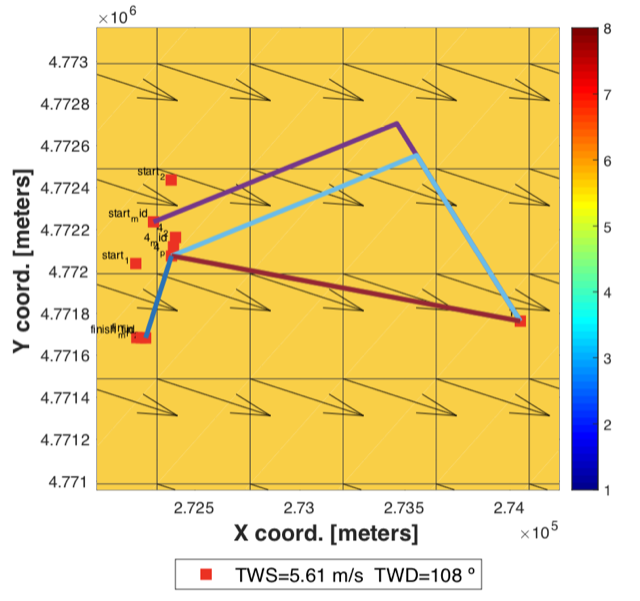
\includegraphics[]{constwind.png}
    %\caption{Minimal Time Trajectory for a Uniform and Constant %wind}
 %   \label{fig:mtp_constWind}
%\end{figure}

\subsection{Constant Wind, Time Step of 60 Minutes (1 Hour)}

In this scenario, the wind field is from the \acrshort{wrf} model, the space grid is 1 km and it remains constant for 60 minutes. This scenario reduced the computational effort since it omits the time dependence because the race has a duration of one hour at the most. The legs on the upwind mode, for this case, shows an alternative direction for the minimal time trajectory compared with the previous scenario. For the leg one, the initial tacking goes to the south and the start point is the midpoint and the one in the north. The leg three in this scenario has more tacking maneuvers and the best path goes to the south also, figure \ref{fig:Windm6_upwind} shows four significant changes in the sailboat's direction. Its pattern follows a zig-zag pattern coming from the south.  \par 

\begin{figure} [hbt!]
  \centering
  \subfloat[Leg 1 trajectories ]{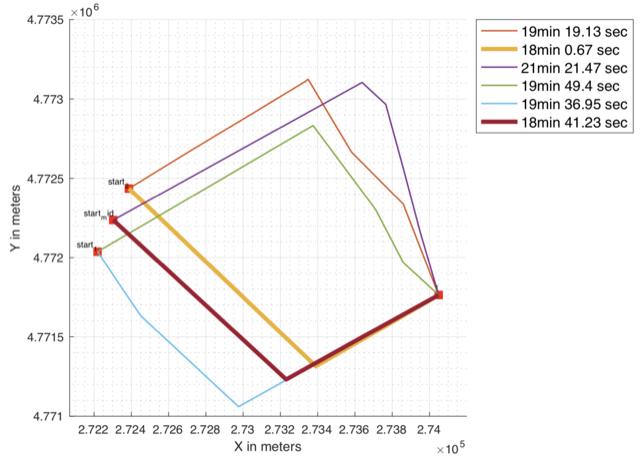
\includegraphics[width=0.43 \linewidth]{images/WindNetCDFm6_Leg1_MC.png} \label{fig:l1_windm6}}
  \hfill
  \subfloat[Leg 3 trajectories] {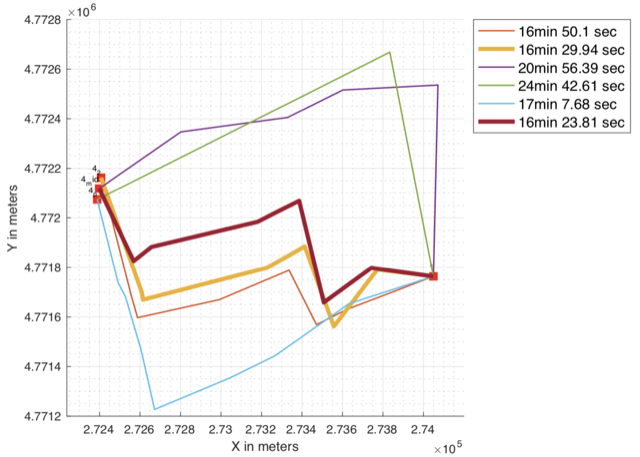
\includegraphics[width=0.44\linewidth]{WindNetCDFm6_Leg3_MC.png} \label{fig:l3_windm6}}
  \caption{Upwind Legs Times from using a wind field constant for 1hr} %$\Delta t$ =5s and
\label{fig:Windm6_upwind}
\end{figure}

The times for both legs on upwind mode for this scenario are larger than in the previous scenario even when the wind conditions reviewed are at 12hrs and at 13hrs. The minimal time trajectory is 54 minutes and 21.97 seconds, the trajectories for each leg are on figure \ref{fig:times_windm6} and for the upwind legs the start locations are the North point for the start and at the midpoint for the third leg. \par 

\begin{figure} [hbt!]
    \centering
    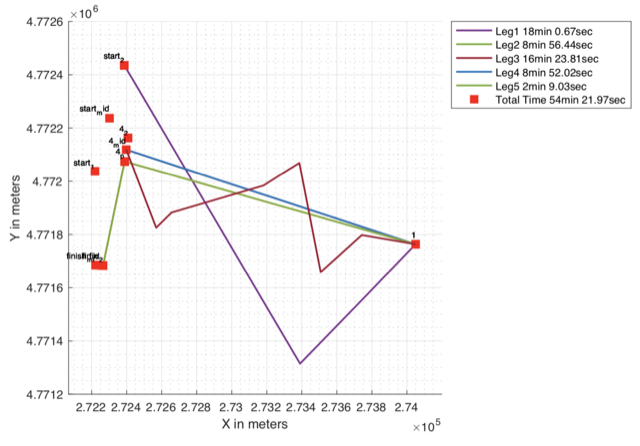
\includegraphics[width=0.75 \linewidth]{WindNetCDFm6_mtp1_MC.png}
    \caption{Total Times and Leg's time for a wind field constant for 1 hr}
    \label{fig:times_windm6}
\end{figure}

The difference of the wind field between the start time and end, are in figure \ref{fig:m6_windprop} where both intensity and direction in average have changed. The direction of the wind has an angle deviation close to 5\degree and at the end, the wind velocity is larger than at the start. The south part of the graph at the end of the race has larger speeds than at the North, while at the start of the race the North had higher wind velocities. This shows how much the velocities can vary over one hour. \par 

\begin{figure} [hbt!]
  \centering
  \subfloat[Total and Legs Times for the race]{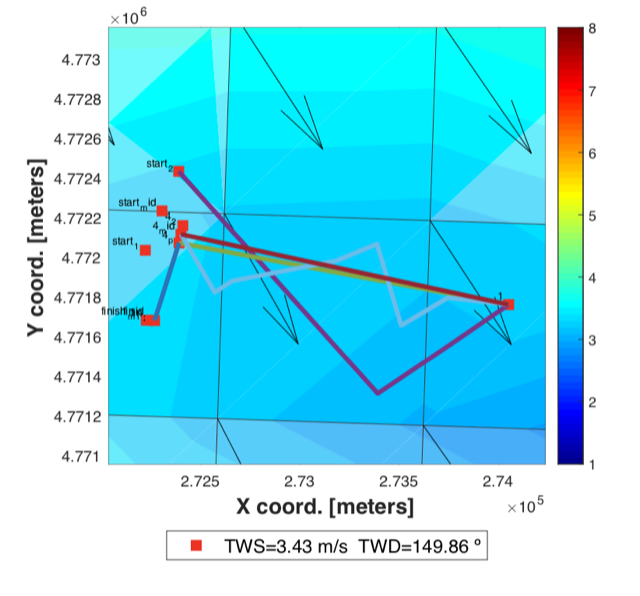
\includegraphics[width=0.46 \linewidth]{images/m6_t0.png} \label{fig:m6_t0}}
  \hfill
  \subfloat[Close up to the Buoys location for R1.] {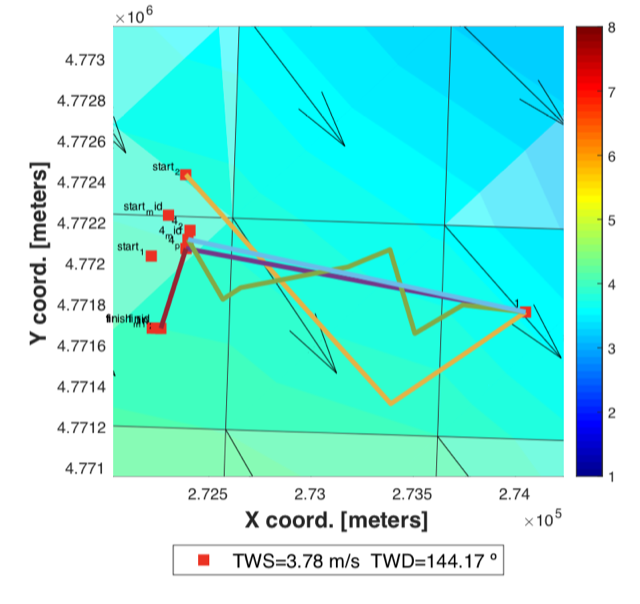
\includegraphics[width=0.46\linewidth]{images/m6_tf.png} \label{fig:m6_tf}}
  \caption{Wind Field at the start and end of the race} %$\Delta t$ =5s and
\label{fig:m6_windprop}
\end{figure}

\subsection{Constant Wind with a Time Step of 30 Minutes (0.5 Hour)}

The parameters of this scenario are like to the previous section, the parameter to vary here is the time step. Here the wind properties remain constant for 0.5 hours or 30 minutes, because of this there is 1 more grid, therefore, one more set of points over time to use, in contrast with the previous section. For the upwind mode the minimal time trajectories show similar directions than the previous scenarios. The best paths of the leg 1 goes to the south, regardless of its start locations point, only one path goes to the north. Furthermore, the top times for the leg 1 start at the North point of the start line and the trajectories overlap in many sections, see figure \ref{fig:l1_windm3}. As a consequence of this, the times differ only by 30 seconds approx, and both trajectories show a zig-zag pattern with at least 3 tacks maneuvers. \par \noindent 

Leg 3 on figure \ref{fig:l3_windm3} shows it has a similar shape than leg 1, here the start point of the two minimal time trajectories are opposite, one starts at the North point while the other is at the South point, however in both cases, they go to the south. \par 

%The legs on the upwind mode, for this case, shows a different direction for the minimal time trajectory. For the leg one, start tacking is to the south and the start point is at the midpoint and the one at the north. The leg three in this scenario has more tacking maneuvers, figure \ref{fig:Windm6_upwind} shows four significant changes in the sailboat's direction. Its pattern follows a zig-zag coming from the south.

\begin{figure} [hbt!]
  \centering
  \subfloat[Leg 1 trajectories ]{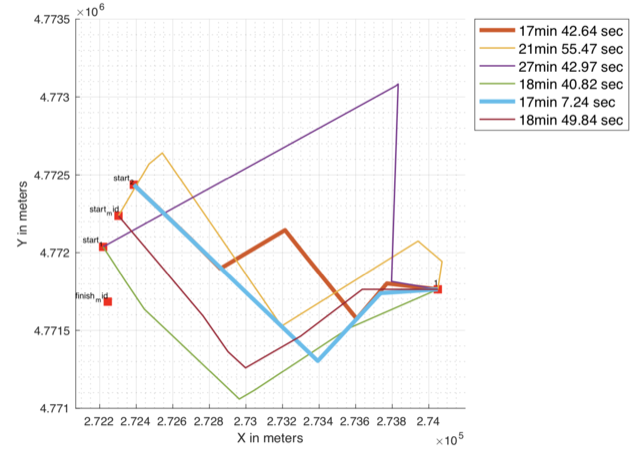
\includegraphics[width=0.43 \linewidth]{images/m3_l1.png} \label{fig:l1_windm3}}
  \hfill
  \subfloat[Leg 3 trajectories] {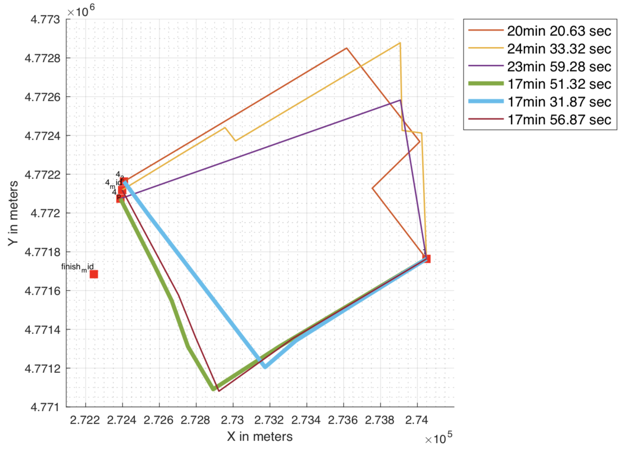
\includegraphics[width=0.44\linewidth]{images/m3_l3.png} \label{fig:l3_windm3}}
  \caption{Upwind Legs Times from using a wind field constant for 0.5hr} %$\Delta t$ =5s and
\label{fig:Windm3_upwind}
\end{figure}

The total time of the race for this scenario is 56 minutes with 31.94 seconds. The times of the leg 1 and 3 are similar, 17 minutes with 7.24 seconds and 17 minutes with 31.87 seconds. Even when the distance of the leg 3 is smaller than the leg 1, it has a longer time trajectory, \ref{fig:times_windm3}. Furthermore, on leg 3, the number of maneuvers is less than at leg 1 and despite this, its time is longer. The downwind mode's legs show  trajectories close to a straight line with tack maneuvers smaller than in the upwind mode. \par  
\begin{figure} [hbt!]
    \centering
    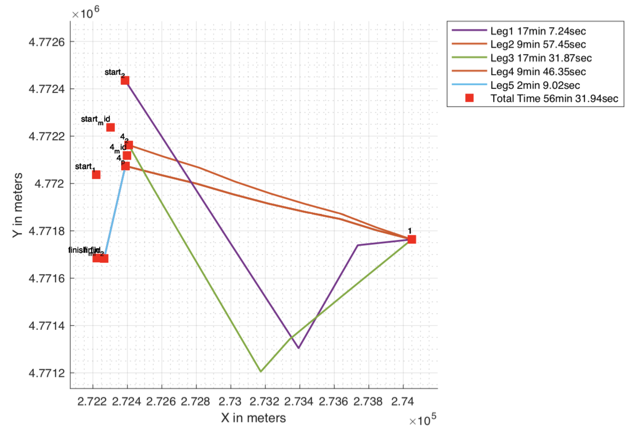
\includegraphics[width=0.75 \linewidth]{images/m3_times.png}
    \caption{Total Times and Leg's time for a wind field constant for 0.5 hr}
    \label{fig:times_windm3}
\end{figure}

The wind properties used on this scenario are from the set points at 12:00 hrs, 12:30 hrs and 13:00 hrs. The wind field pattern at these times is in figure \ref{fig:m3_wind}. The figure \ref{fig:m3_tm} shows the transition between speeds, the top side has lower velocities than the bottom side. The wind shift directions between the three of them are approx. 2 \degree. The resultant trajectory of this scenario and the previous one are  different, not only in time but in shape also. In this scenario, the number of tacks is less than with a wind constant for one hour however the time is longer than it. For the leg 3 even when the wind is stronger, the variation on its angle is larger than at the end.  \par    

\begin{figure} [hbt!]
  \centering
  \subfloat[Wind Field at 12:00 hrs ]{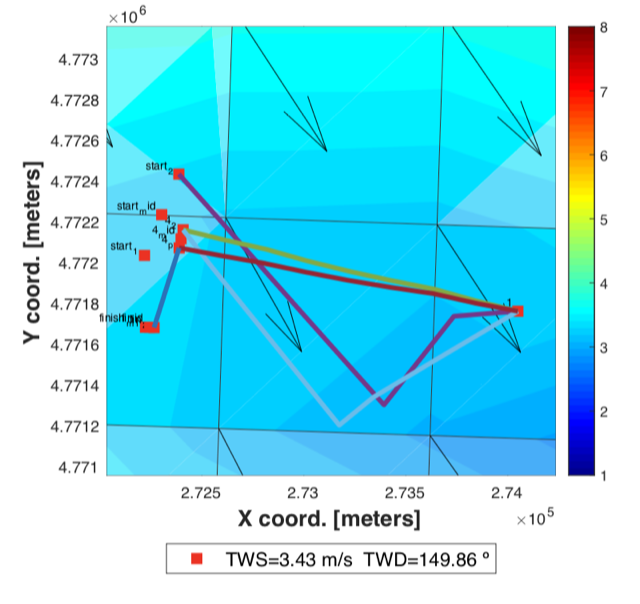
\includegraphics[width=0.32 \linewidth]{images/m3_t0.png} \label{fig:m3_t0}}
  \hfill
  \subfloat[Wind Field at 12:30 hrs] {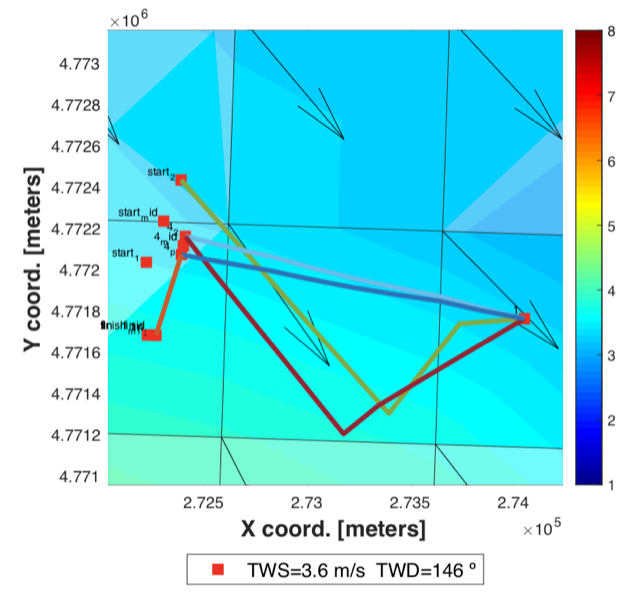
\includegraphics[width=0.32\linewidth]{images/m3_tm.png} \label{fig:m3_tm}}
    \hfill
  \subfloat[Wind Field at 13:00 hrs.] {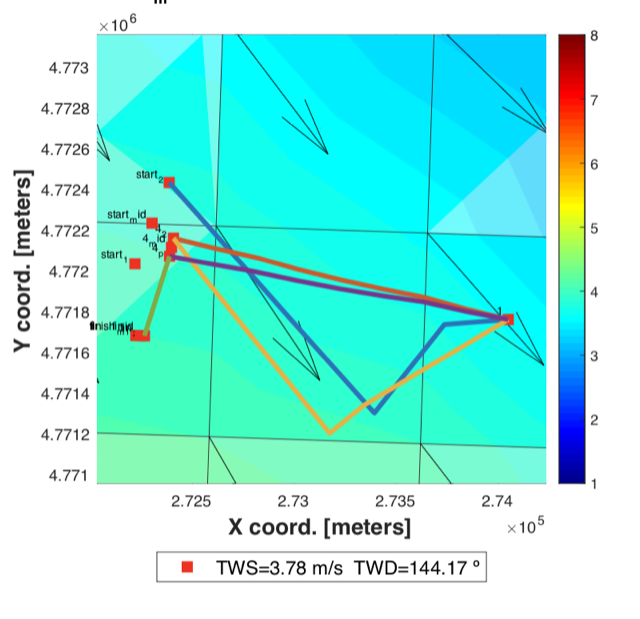
\includegraphics[width=0.32\linewidth]{images/m3_tf.png} \label{fig:m3_tf}}
  \caption{Wind Field properties, variation over time} %$\Delta t$ =5s and
\label{fig:m3_wind}
\end{figure}

\subsection{Wind field with a Time Step of 10 Minutes (1/6 Hour)}

This scenario uses the \acrshort{wrf} wind model as it is, where the wind field varies in space and time. The time step is 10 minutes, or 600 and a grid size about 1 km by side. %seconds this means that the wind's velocities are constant for 10 minutes. 
As a result of this, the number of grid points increased significantly, and consequently the  computational effort. \par

For the upwind legs, figure \ref{fig:Windnetcdf_upwind} shows that the top minimal trajectories for both legs follow to the south. For example, the start point of leg 1 is one in the middle and the other in the south. The path that starts at the middle point has more shifts in direction than the other path and it arrives in the next buoys with a final tack to the south. The other path which is the second-best initially goes to the south and then shifts direction to the north. The variation in time between them is only about 16 seconds. \par \noindent 

For leg 3, the top minimal time trajectories both starts at the north point and both go to the south. The best of them have an "L" pattern instead of a zig-zag such as in the second best path. The difference in time between them is 1 minute and in this case, this difference is more related to the number of shifts. Moreover, most of the trajectories despite where they start, they go to the south except for one which also has the largest time among them. \par  % This means that different start points converge to one direction, however the time of each of them depends on the number and distance at which they shift direction. \par 

\begin{figure} [hbt!]
  \centering
  \subfloat[Leg 1 trajectories ]{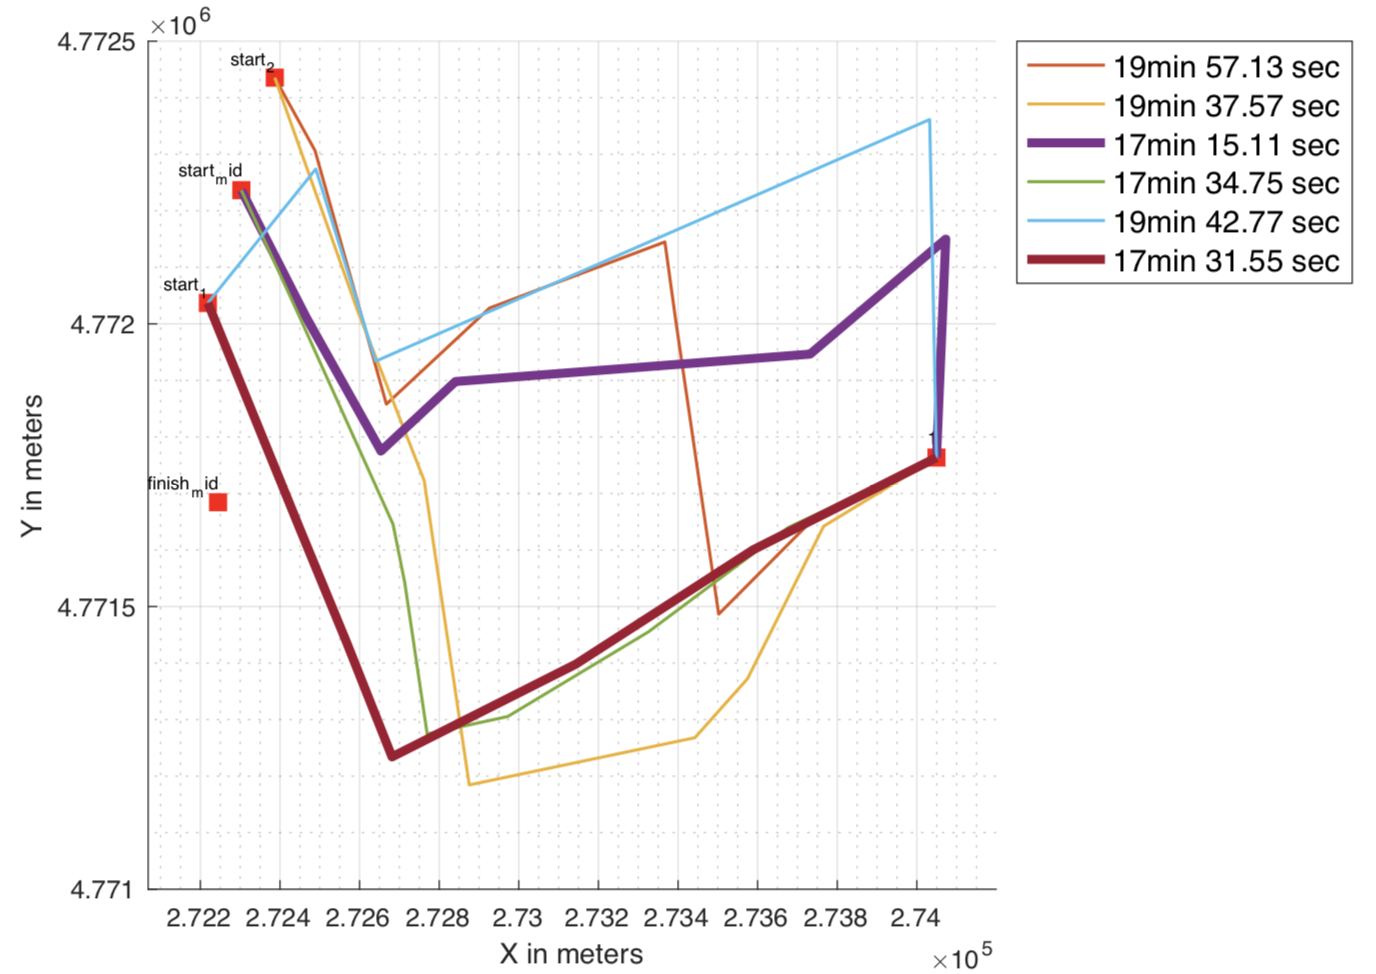
\includegraphics[width=0.41 \linewidth] {images/netcdf_l1.png}  \label{fig:l1_windnetcdf}}
  \hfill
  \subfloat[Leg 3 trajectories]  {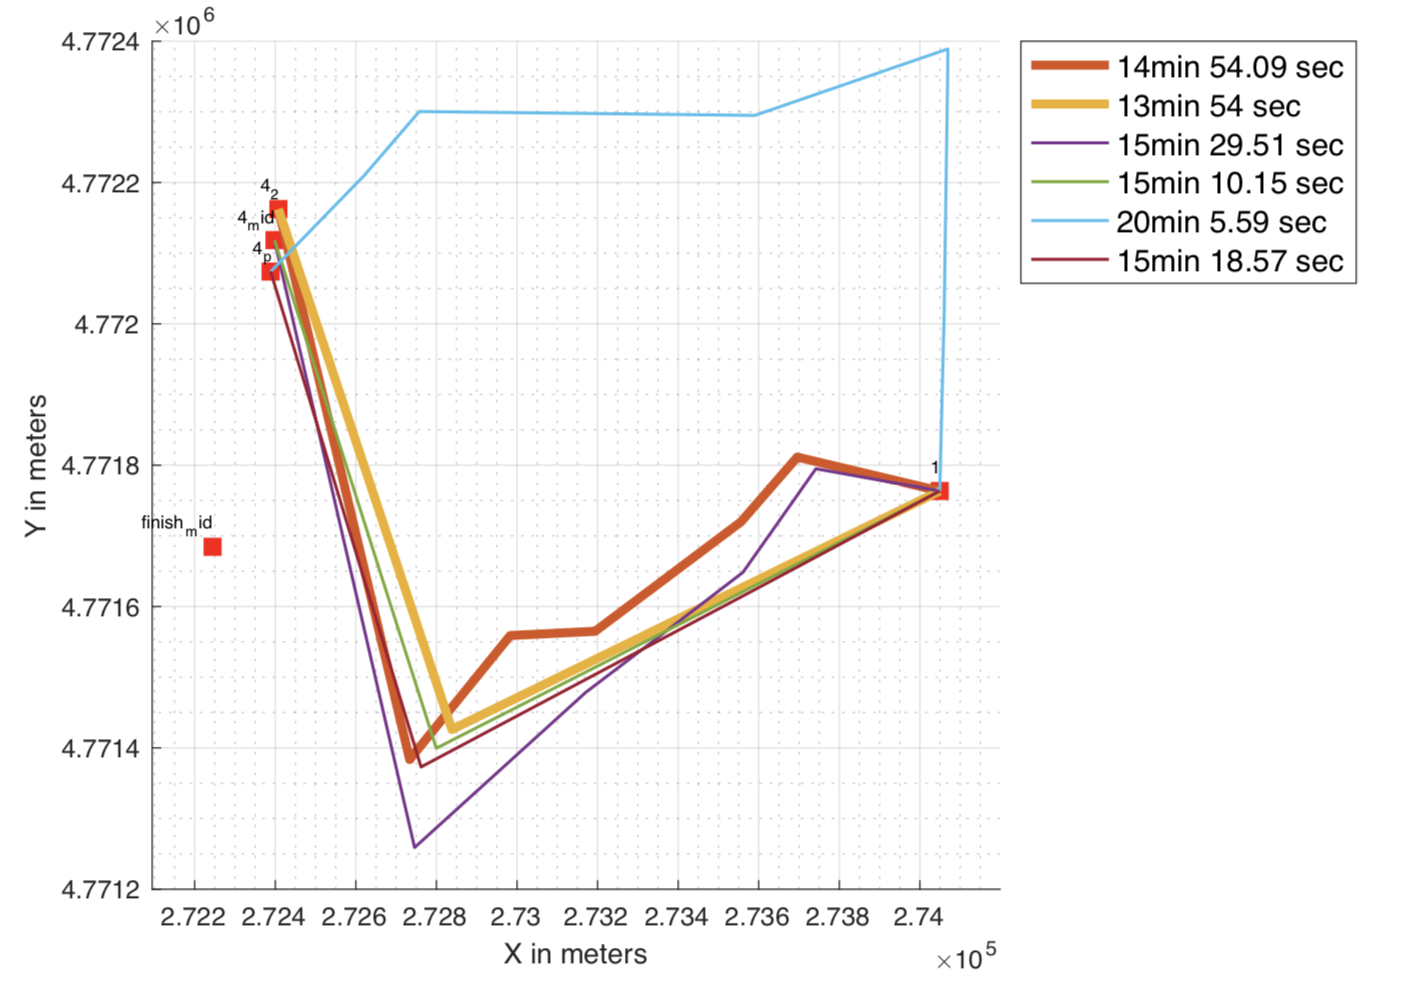
\includegraphics[width=0.41\linewidth]{images/netcdf_l3.png} \label{fig:l3_windnetcdf}}
  \caption{Upwind Legs using the WRF wind model with a time step of 10 minutes.} %$\Delta t$ =5s and
\label{fig:Windnetcdf_upwind}
\end{figure}

The total time in this scenario is 51 minutes and 11.97 seconds until know it is the smallest time. The minimal time's trajectories for the upwind-mode starts at the mid and north point of the respective line. The leg 1 is the leg with the most tack maneuvers in contrast with the rest of the legs as a consequence its time is the largest. The rest of the legs do not follow properly a zig-zag pattern, leg 3 as mentioned before, follows an "L" shape  with the one tack maneuver, the rest of the legs follows a straight line, therefore, the resulting path is figure \ref{fig:times_windnetcdf}. \par  

\begin{figure} [hbt!]
    \centering
    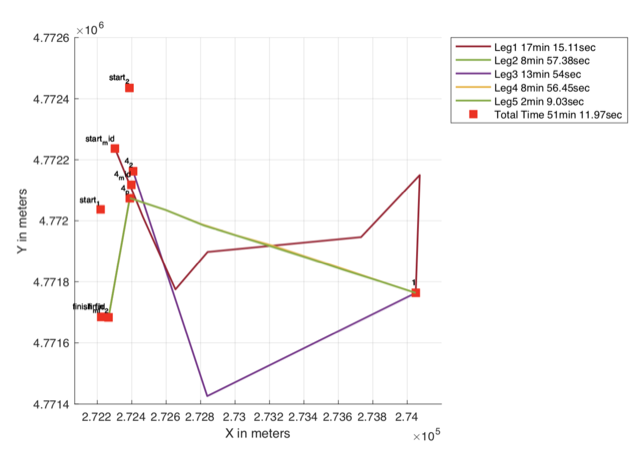
\includegraphics[width=0.75 \linewidth]{images/netcdf_times.png}
    \caption{Minimal Time Path using the WRF model with a step time of 10 minutes}
    \label{fig:times_windnetcdf}
\end{figure}

Because more grid data points are available, the wind field variation is more accurately. For comparison purposes,figure \ref{fig:netcdf_wind} only shows 3 steps, these set of points are at 12:10 hrs, 12:20 hrs and 12:40 hrs, in fact, the wind properties for 12:30 hrs and 13:00 hrs are the same as in figure \ref{fig:m3_tm} and \ref{fig:m3_tf}. Comparing figure \ref{fig:netcdf_t10} with figure \ref{fig:netcdf_t20} the winds speed  (\acrshort{v_tw}) increases while the wind angle (\acrshort{b_tw}) decreases.  %the  however this difference is insignificant due to the size of the area is not perceptible. 

\begin{figure} [hbt!]
  \centering
  \subfloat[Wind Field at 12:10 hrs ] {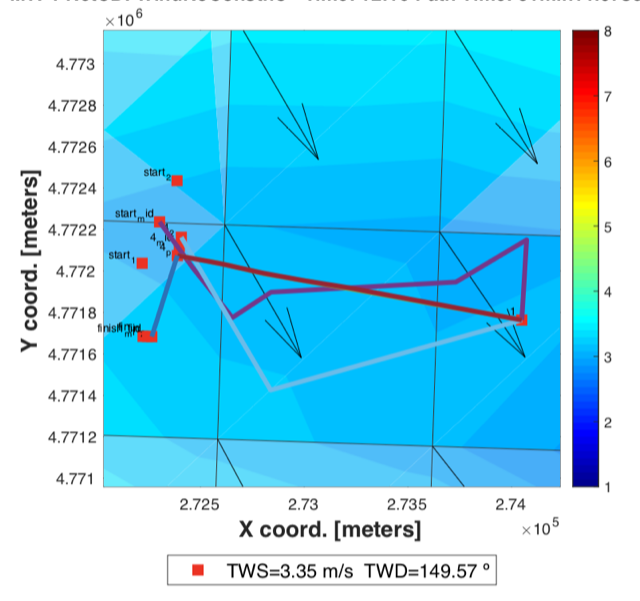
\includegraphics[width=0.32 \linewidth]{images/netcdf_tm.png} \label{fig:netcdf_t10}}
  \hfill
  \subfloat[Wind Field at 12:20 hrs] {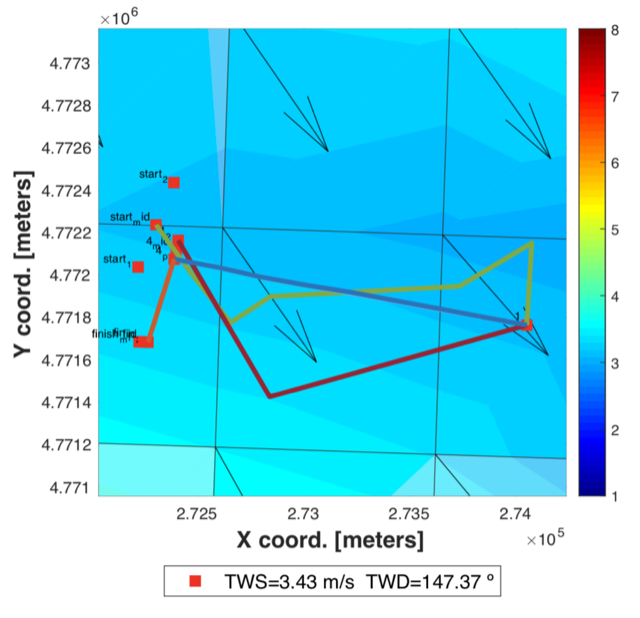
\includegraphics[width=0.32\linewidth]{images/netcdf_t20.png} \label{fig:netcdf_t20}}
    \hfill
  \subfloat[Wind Field at 12:40 hrs.] {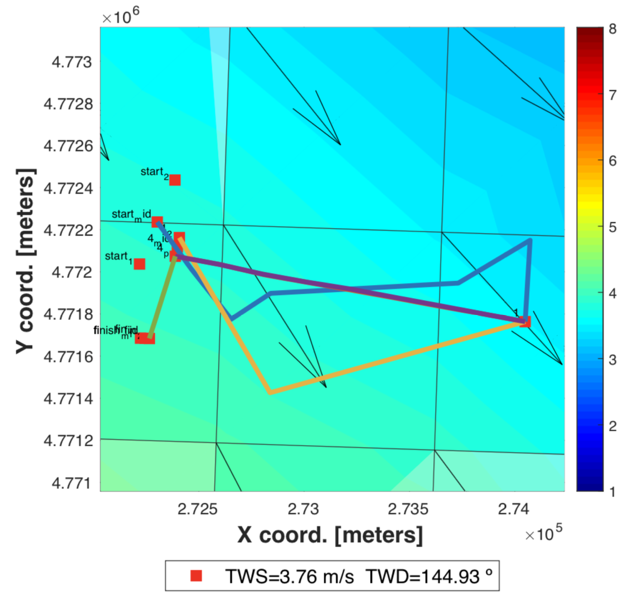
\includegraphics[width=0.32\linewidth]{images/netcdf_t40.png} \label{fig:netcdf_t40}}
  \caption{Wind Field changes over time from the WRF model.} 
\label{fig:netcdf_wind}
\end{figure}

\subsection{Wind Measurements from the Race}
In this scenario, the wind data is from the race, where the sampling rate was 20 HZ and it comes from  5 locations dispersed around the courses areas. These measurements were at a height of 7.5 meters approx. so the algorithm converted to the \acrshort{ce} height, similarly as in with previous scenarios. \par \noindent
The upwind legs for this scenarios show opposite directions to follow in contrast with previous scenarios particularly for the leg 1. Figure \ref{fig:sap_upwind} also shows that the times are larger than the previous results. The preferable start direction remains to be the midpoint  and  the north point. The best times start at distinct points going to the north and then do a significant shift to the heading direction to go to the buoy at its south. In fact, this last shift makes that both paths coincide until it arrives to the next buoy.\par \noindent  
leg 3 has a similar pattern than previous sections an "L" or "V" shape with small tacking maneuvers in between. The best path starts at the south point while the second-best start at the middle point, the time difference between them is about 19 seconds. In this leg, all the half of the paths go to the north and the other to the south, in both cases all paths have a "V" shape.   \par 

\begin{figure} [hbt!] 
  \centering
  \subfloat[Leg 1 trajectories ]{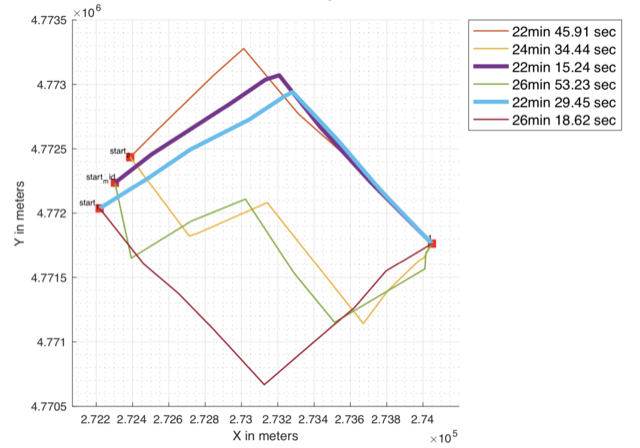
\includegraphics[width=0.43 \linewidth] {WindSap_Leg1_mC.jpg}  \label{fig:sap_l1}}
  \hfill
  \subfloat[Leg 3 trajectories]  {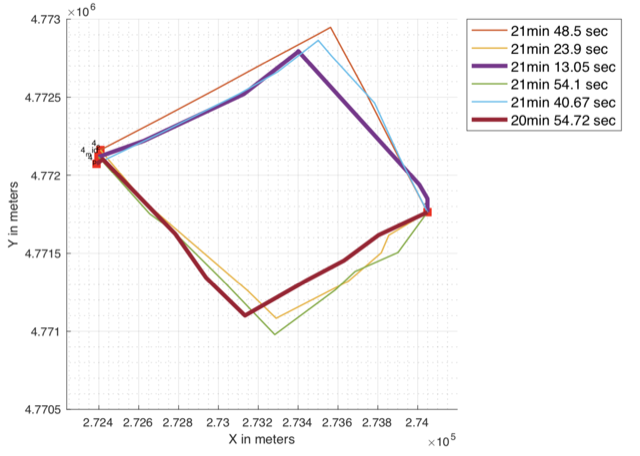
\includegraphics[width=0.43\linewidth]{images//WindSap_Leg3_mC.jpg} \label{fig:sap_l3}}
  \caption{Upwind Legs Times from using the WRF wind model with a time step of 10 minutes (1/6 hrs)} %$\Delta t$ =5s and
\label{fig:sap_upwind}
\end{figure}

Figure \ref{fig:times_winSAP} shows the minimal time path for this scenario, the upwind sailing legs have a "V" shape while the rest of the legs sail in a straight line direction. The total time of the race is 63 minutes and 42.35 seconds, this time is much larger than previous results. \par  

\begin{figure} [hbt!]
    \centering
    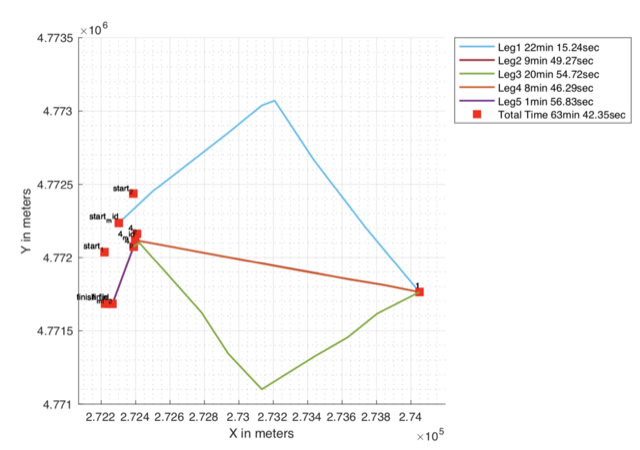
\includegraphics[width=0.75 \linewidth]{images/WindSap_mtp1_angConst.png}
    \caption{Total Times and Leg's time using the WRF model with a step time of 10 minutes or (1/6 hr)}
    \label{fig:times_winSAP}
\end{figure}

The wind field for this scenario does not have a grid size as the \acrshort{wrf} wind model. The wind velocities are larger but with a wind direction smaller than the previous scenarios, this wind direction is close to 100\degree in contrast with the 144\degree from the \acrshort{wrf} model.  The variation of the wind at the start of the race at 12:10 hrs, 12:30hrs and 13:00 hrs are in figure \ref{fig:sap_prop}. \par 

\begin{figure} [hbt!]
  \centering
  \subfloat[Wind Field at 12:10 hrs ]{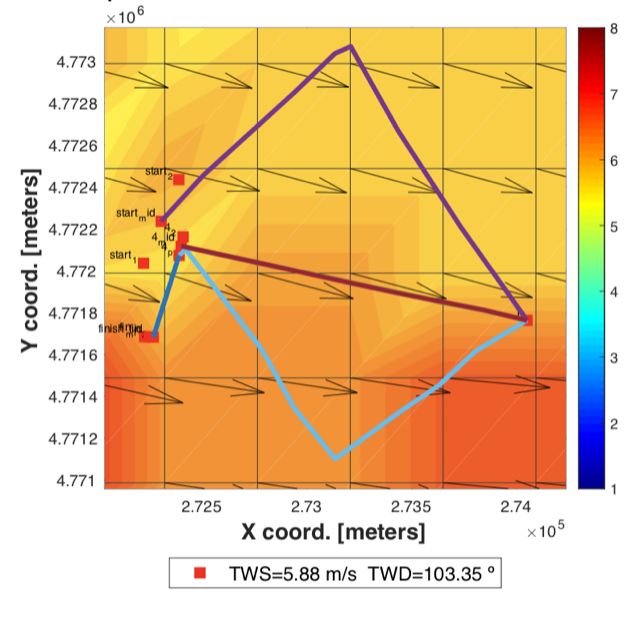
\includegraphics[width=0.31 \linewidth]{images/sap_t0.png} \label{fig:sap_t0}}
  \hfill
  \subfloat[Wind Field at 12:30 hrs] {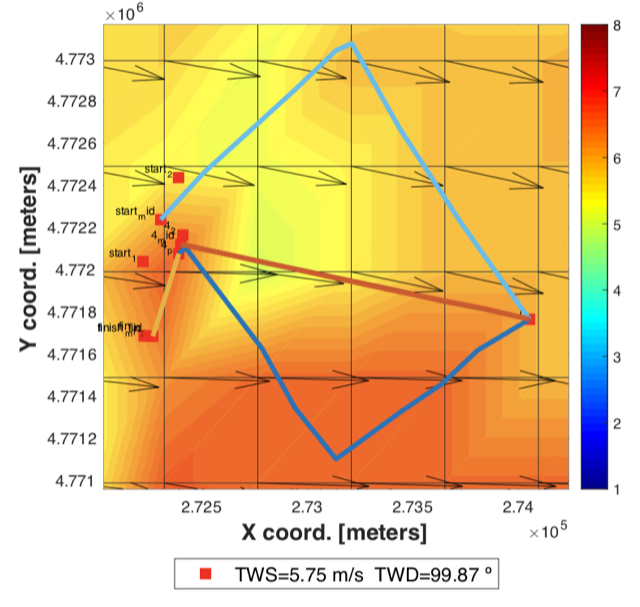
\includegraphics[width=0.32\linewidth]{images/sap_tm.png} \label{fig:sap_tm}}
    \hfill
  \subfloat[Wind Field at 13:00 hrs.] {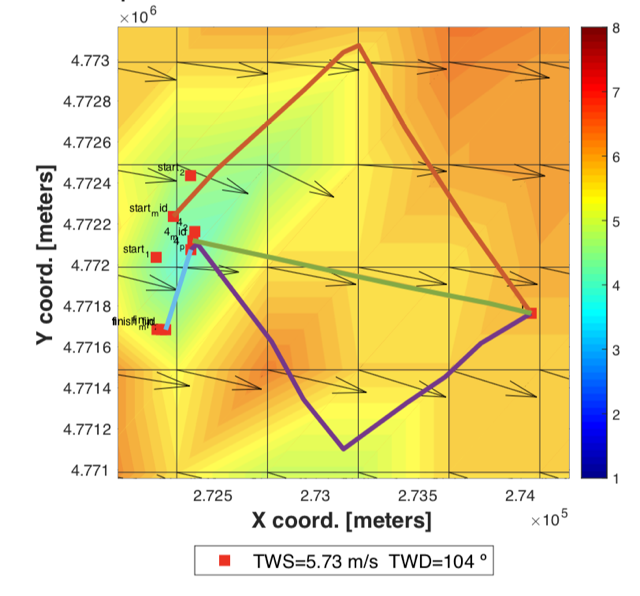
\includegraphics[width=0.33\linewidth]{images/sap_tf.png} \label{fig:sap_tf}}
  \caption{Wind Field from race measurements}
\label{fig:sap_prop}
\end{figure}

Moreover, the wind speed (\acrshort{v_tw}) and direction(\acrshort{b_tw}) over the racecourse R1 varies over time following a different pattern compared with the \acrshort{wrf} wind model. For example, at the end of the race 13:00 hrs figure \ref{fig:sap_tf} and \ref{fig:m3_tf} show the wind speed varies between 5 and 4 m/s. Figure \ref{fig:sapWind_locations} shows the locations of the race measurements with blue dots and its wind field properties. The spatial distribution of these locations are not uniform and the locations of many of the points for R1 and other courses are far from them. Meanwhile, many of the measurements are closer to the center of the \textit{Echo} course thus, this algorithm estimated the wind properties of the race-lines via interpolation.%and how these measurements estimate the wind properties. 
Using the locations of the grid points from the \acrshort{wrf} at 12:00 hrs figure \ref{fig:winds_mod_comp} shows both wind fields. The wind speeds (\acrshort{v_tw}) and the wind's angle (\acrshort{b_tw}) of each is different furthermore, the wind properties of most of these points-locations results from an extrapolation method. %have wind properties are extrapolated to estimate the wind properties at any time. 
This extrapolation especially influences the upwind modes, in other words, the conditions at which the wind sail at leg 1 and leg 3. These variations, particularly on the direction, are the reason why the paths have a different shape and form. \par 

%\begin{figure} [hbt!]
 % \centering
 %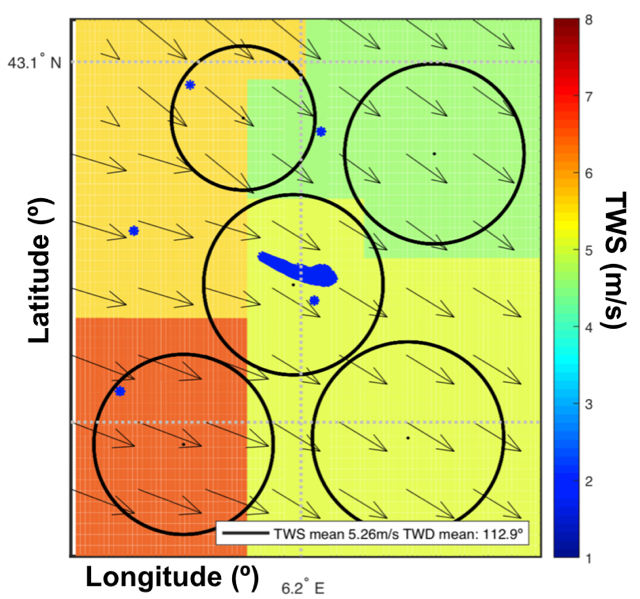
\includegraphics[width=0.4 \linewidth]{sap_wrf.png} 
 % \caption{Wind Measurements locations from the WRF Model.} %$\Delta t$ =5s and
%\label{fig:sapWind_locations}
%\end{figure}

\begin{figure} [hbt!]
  \centering
  \subfloat[Wind Measurements locations the wind field estimated using the WRF grid locations. ]{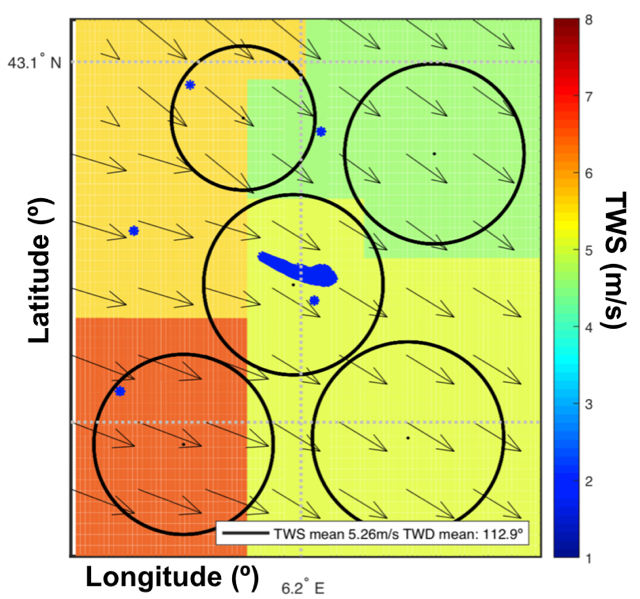
\includegraphics[width=0.45 \linewidth]{sap_wrf.png} \label{fig:sapWind_locations}}
  \hfill
  \subfloat[WRF wind Field ] {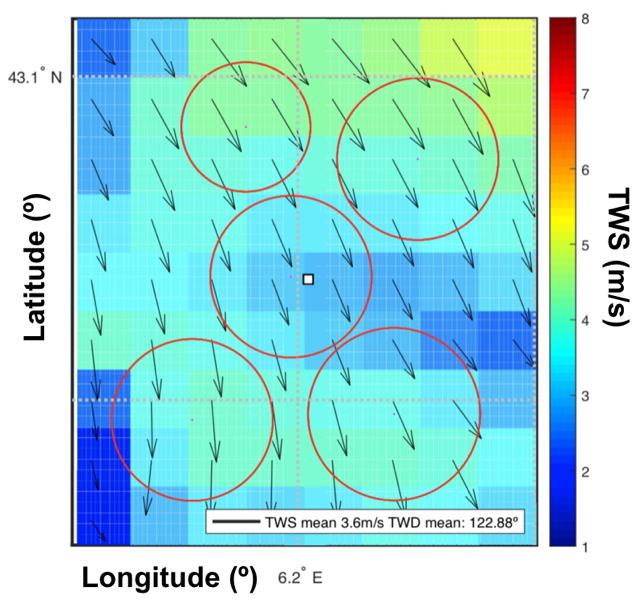
\includegraphics[width=0.44\linewidth]{images/wrf2.png} \label{fig:wrf_wmodel}}
  \caption{Wind Field from race measurements and WRF wind field at 12:10 hrs.}
\label{fig:winds_mod_comp}
\end{figure}


\section{Comparison of the Results with the Winners Race}

In this section,  I compare the results of the previous scenarios with the results from the race. For this, only the top 10 winners are considered for the analysis. The \textit{SAP Sailing Analytics}\textsuperscript{\textregistered} website provides the information about to the times and paths. The comparison uses the times and paths. In the case of the times, the comparison uses the legs times and the race-time. The units used for the time are seconds and the order used is the same as the one from the scenario's section.\par 

\begin{figure}[htb!] 
    \centering
    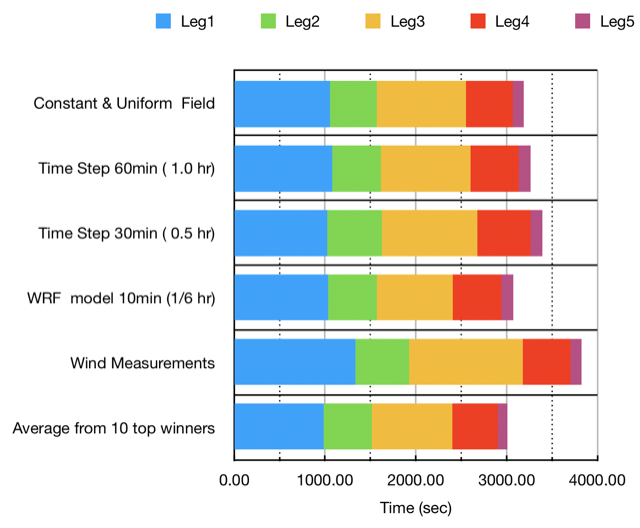
\includegraphics[width=0.6\linewidth]{TimesComparionsFilesg.png}
    \caption{Times Legs by scenario and the average time of the top 10 winners for the race}
    \label{fig:TimeLegs}
\end{figure}

The summation of the duration of each leg results in the race-time. The collection of all the race times and legs got from the scenarios previously showed are in figure \ref{fig:TimeLegs}. In this figure, \textit{Wind Measurements} refers to the results using the wind measurements from the race. Comparing the legs times from each scenario against the average from the top 10 winners shows that the first leg except the wind measurements results is similar. Furthermore, leg 3 also sailing in upwind mode has a duration smaller than leg 1 and this condition only occurs in the \acrshort{wrf} wind model. \par 

\begin{figure}[htb!] 
    \centering
    \includegraphics{images/TimesLEGS_Race.png}
    \caption{Timess by Legs according the scenerios}
    \label{fig:timesLegs_Sce}
\end{figure}

When the leg times comparison is only for the \acrshort{wrf} wind model, the average of the top 10 winners and the winner of the race. The leg 5 is significantly shorter in contrast with the resulted leg from the \acrshort{wrf} wind model scenario, figure \ref{fig:TimeTopComp} shows this. Moreover, this leg according to the results from previous sections was sailing in a straight line, similarly happens to the leg 4. \par 

\begin{figure}[hbt!] 
    \centering
    \includegraphics[width=0.6\linewidth]{images/TimesComparionsTop.png}
    \caption{Leg's Times comparisons for the winners and the WRF wind field scenario.}
    \label{fig:TimeTopComp}
\end{figure}

The detailed comparison between the average results from the top 10 winners and the \acrshort{wrf} wind model results are in figure \ref{fig:table10WinnerComp}. This shows that the race time difference between both results are close to 62 seconds, and this represents an error of -2\% from the average race result of the top 10 winners. Furthermore, the leg 5 has the largest percentage error which is 17\% while the smallest error is for leg 2 with 1.75\%. In fact, the rest of the legs have a percentage error  between 4.75\% and 6.28\%.

\begin{figure}[hbt!] 
    \centering
    \includegraphics[width=0.95\linewidth]{images/table_comp_W10winner.png}
    \caption{Time Comparison by leg between the WRF wind results and the average of the top 10 winners.}
    \label{fig:table10WinnerComp}
\end{figure}

When the detailed comparison is between the \acrshort{wrf} wind model and the winner of the race. The variations for the race time shows a time difference about 130.97 seconds which represents 4.26\%, in fact, this error is double compared with the average of the top 10 winners of the race. The error for the leg 5 are still 17.85\% additionally the error percentage for leg 4 is in this case 10.52\%  and for leg 2 it is 6.96\%. The rest of the legs have an error of around 4\% approx.\par  

\begin{figure}[hbt!] 
    \centering
    \includegraphics[width=0.95\linewidth]{images/table_comp_Wwinner.png}
    \caption{Time Comparison by leg between the WRF wind results and the winner of the race.}
    \label{fig:tableWinnerComp}
\end{figure}

Another aspect to review after the times is the shape of the minimal time resulting from the scenarios and the developed paths from the race, these are in figure \ref{fig:PathSimulations_topten}. For this, the comparison uses again the top ten competitors. The results from the top ten competitors show that the winners followed a north direction when the race starts for the upwind mode legs. In the other hand, for the downwind mode legs they do not follow a straight-line path as in the last case. Instead, they follow an alternative shape which neither looks like a zig-zag pattern. The simulation's results show for the upwind-mode paths that go to the north and south and straight lines paths for the downwind mode legs and the last leg.\par 
\begin{figure} [hbt!]
  \centering
  \subfloat[Simulations Paths ]{\includegraphics[width=0.32 \linewidth]{images/PathCompScenarios.png} \label{fig:SimulationsPathsTraj1}}
  \hfill
  \subfloat[Top Ten Winners ] {\includegraphics[width=0.32\linewidth]{images/Top10Comp.png} \label{fig:TopTenPaths}}
  \hfill
  \subfloat[Top 3 Winners ] {\includegraphics[width=0.32\linewidth]{images/Top3Comp.png} \label{fig:Top3Paths}}
  \caption{Wind Field from race measurements and WRF wind field at 12:10 hrs.}
\label{fig:PathSimulations_topten}
\end{figure}
If the comparison from the race only uses the top three winners as in figure \ref{fig:Top3Paths} it shows that the downwind mode legs follow a path that has a shape of a curve. The winner of the race on the upwind mode legs has a larger length trajectory and for the downwind-mode, its trajectory is not a straight line. Besides this, the start points for the upwind-mode shows that for leg 1 the 3 winners starts around the midpoint. In contrast, for leg 3, the winner goes to the north point while the other two winners went to the south point. In these comparisons, it can see that the downwind mode legs follow path trajectories that contrast from the shaped developed by  the scenarios.\par 

To clarify the differences between the shapes from the scenarios and the shape of the winner, the paths are in the same plot. The first path scenario results from the constant and uniform wind field, figure \ref{fig:winnerConstUnif} displays this. Leg 3, leg 4 and leg 5 coincide with the path followed by the winner. The leg 1 from the scenario goes to the north and it starts at the middle point similarly as the winner did. However, this leg does not coincide as the legs mentioned before. \par 

\begin{figure}[hbt!]
    \centering
    \includegraphics[width=1\linewidth]{images/WinnerConst1200.png}
    \caption{Constant and Uniform Wind Resulting race path and the winner's path}
    \label{fig:winnerConstUnif}
\end{figure}

In the case of the path resulting from the \acrshort{wrf} wind model, the legs do not coincide with the paths trajectories from the winner except for the last two legs, leg 4 and 5, this is displayed in figure \ref{fig:WRF_Winner_start}. However, the start point for the upwind legs coincide. As mentioned before the time difference of the total race is only 130.97 seconds or 4.26 and despite that the leg 5 has the same path trajectory its times are different. Same happens with the leg 4 and in both cases, the error is about 17.85\% and 10.53\% respectively. \par 

\begin{figure}[hbt!]
    \centering
    \includegraphics[width=1\linewidth]{images/WinnerNet1210.png}
    \caption{WRF Wind's resulting race path and the winner's path}
    \label{fig:WRF_Winner_start}
\end{figure}

When the resulting race path from the wind measurements is compared with the path trajectory of the winner's race.  Figure \ref{fig:Sap_Winner_start} displays that the last 2 legs coincide with the winner's path, this is not the case for the legs sailing under upwind-mode. Particularly, the leg 3 unlike the last two legs, this leg's path sails in the opposite direction than the winner, it sails to the south while the winner sails to the north. Leg 1, in both cases, has a "V" shape and it also starts at the middle point. Moreover, the trajectory after the first tack maneuver is similar. The time for the last two legs are 10.83 and 46.29 seconds for the leg 5 and leg 4 respectively, these differences represent approximately 10\% from the winner's leg's times. \par   

\begin{figure}[t]
    \centering
    \includegraphics[width=1\linewidth]{WinnerSap1210.png}
    \caption{Wind measurement's field resulting race path and the winner's path}
    \label{fig:Sap_Winner_start}
\end{figure}

This section describes the results and how the time window and buoys locations from the race defines the parameters of the optimization algorithm. As a result of this, the algorithm solve the minimal time path for a variety of scenarios.   %were used to finish the resulting paths from different wind field scenarios and compare 
Furthermore, using the winner's race times and path  and contrasting with the results from the scenarios they show the differences and similarities between them. This comparison uses most of the time the average of the top ten winners. The comparison of the shape shows sometimes contrasting results. In addition, the evolution of the wind during the race shows the variations over the path development and how these influences its shape. 
%Thus when only the time results were reviewed and at the same time how the wind field evolve from the start of the race to its end. 
The next section is for the conclusion and recommendations of this research. \par 

